% ============================================================
% Sección 0: Sobre mí (línea de tiempo de trayectoria)
% ============================================================

\begin{frame}{Sobre mí: trayectoria}
  \centering
  \begin{tikzpicture}[
      every node/.style={font=\scriptsize},
      etapa/.style={align=center, text width=1.9cm, font=\scriptsize}
    ]
    \draw[flecha, line width=1pt] (0,0) -- (12,0);

    \foreach \x/\lbl/\txt in {
        0/{2004}/{Lic. en Física\\(U. de Guadalajara)},
        2/{2007-13}/{MSc y PhD\\(UNAM / CINVESTAV)},
        4/{2017-18}/{Postdoc HPC+IA\\(Barcelona SC)},
        6/{2019-24}/{Director IA\\Gob. de Jalisco},
        8/{2020}/{Fulbright-García\\Robles (UT Dallas)},
        10/{2022-hoy}/{Consultor IA\\(World Bank, ...)},
        12/{2025-hoy}/{Director IA-HPC\\(IIEG)}
      }{
        \node[nodoTiempo] at (\x,0) {};
        \node[etapa, above=0.3cm] at (\x,0.3) {\lbl};
        \node[etapa] at (\x,-1.1) {\txt};
      }
  \end{tikzpicture}

  \vfill
  \small
  Ph.D. en Ingeniería Eléctrica · +65 publicaciones en IA para salud, clima y NLP \\
  Top 10 UNESCO-IRCAI Global 100 · Proyectos con OECD-GPAI, Banco Mundial y ONU
\end{frame}


\begin{frame}{Equipo de Trabajo}
\begin{center}
  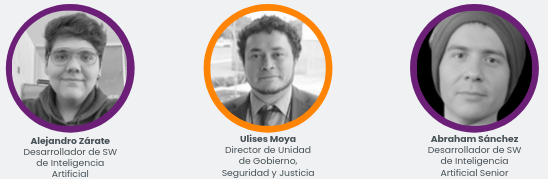
\includegraphics[width=0.45\paperwidth,height=0.38\paperheight,keepaspectratio]{images/team.png}
\end{center}
\end{frame}
